\section{Analysis and Implementation of Attack Vectors}
\label{sec:attack}

In this section, we detail our novel attack vectors targeting the EEG system framework demystified in Section~\ref{sec:framework}. Our attack vectors can be classified as either remote attacks or proximate attack. In a remote attack, an attacker can launch the attack without any constraint on how far he is away from the victim; however, a carefully crafted malicious program residing in the victim's PC side \emph{is} required to run. In a proximate attack, on the other hand, an attacker has to launch the attack within a certain distance away from the victim; however, \emph{no} malicious app is needed in this case. %Therefore, an attacker can freely choose any of the two types of attacks to launch based on different situations.

\subsection{Remote Attacks}
We came up with four remote attack cases based on the roles a malicious program plays in the EEG system framework: as a malicious BCI app, as a malicious TGSP server, or as a malicious SDK. We have fully implemented these attacks. 

\subsubsection{Malicious Program as a BCI App}
The most straightforward attack is to install a malicious BCI app which secretly steals a victim's EEG data. As described in Section~\ref{sec:framework}, a BCI app can retrieve EEG data through either the standard SDK or TGSP. Correspondingly, there could be two approaches to implement such a malicious program. \\
\indent \textbf{Exploiting Standard SDK:} We first analyzed  if it is possible to implement a malicious BCI app which steals the victim's EEG data by exploiting the standard SDK. After an initial exploration, we found that if there is no other BCI apps running, our malicious app can successfully retrieve the EEG data; however, if there is another BCI app running, this method fails. We then  conducted dynamic debugging on the binary \texttt{thinkgear.dll} and found that when a BCI app calls \texttt{TG\_Connect}, \texttt{TG\_Connect} calls a sub function which invokes \texttt{CreateFileA} in Windows \texttt{kernel32.dll} and passes the fixed name of the RF dongle serial port, e.g., ``COM3'', as the file name to \texttt{CreateFileA}. Therefore, when a BCI app is accessing the serial port through SDK, another app would fail since \texttt{CreateFileA} would return the \texttt{ACCESS\_DENIED} error. Hence, through this method, a malicious app would have to terminate the benign program running a BCI app or the TGSP server (which is basically a BCI app), if any, in order to accomplish the attack. Intuitively, terminating a running benign app can trigger a victim's suspicion. Hence, a malicious app has to imitate the terminated benign app at every level, imposing a tremendous burden to the attacker. \\
\indent \textbf{Exploiting TGSP:} A relatively easy approach is to exploit TGSP; thus we examined the feasibility of a malicious BCI app accessing the EEG data through TGSP. As we mentioned in Section~\ref{sec:framework}, the TGSP server adopts a naive verification step merely for the purpose of distinguishing different apps. Therefore, we implemented a malicious app using C/C++ which generates a random string as the app name, constructs a SHA-1 digest for the app name, and sends these two pieces of information to TGC. If there is a conflict, our malicious app simply re-generates another random app name. It turns out that this attack functions normally.

\subsubsection{Malicious Program as a TGSP Server}
Instead of creating a malicious BCI app, we also created a malicious program which acts as a fake TGSP server and responds to benign BCI apps while retrieving the EEG data using the standard SDK. Note that even though this attack is refined based on the previous attack, it is more complicated since it needs to maintain TGSP so that benign BCI apps can run normally.\\
\indent In order for this attack to operate successfully, we first need to terminate the legitimate TGSP server, TGC, if it is running. TGC is not executed at the administrator level so that it can be terminated easily by calling the Windows Kernel API \texttt{TerminateProcess}. Then our malicious server maintains the TGSP specifications as we described in Section~\ref{sec:framework}. This attack is fully implemented in C/C++.

\subsubsection{Malicious Program as SDK}
Besides the attacks mentioned above, we also constructed an attack by modifying the standard SDK into a malicious one. In Section~\ref{sec:framework}, we identified the 4 mandatory API functions in \texttt{thinkgear.dll} to complete the EEG data retrieval. Among these 4 functions, the most important one is \texttt{TG\_GetValue} since it returns the requested EEG data. Hence, directly attacking this function in \texttt{thinkgear.dll} is the simplest and most effective way to steal the EEG data. \\
%
\indent In order to modify \texttt{TG\_GetValue}, we had to dig into the detailed specification of the function. \texttt{TG\_GetValue} is defined in the \texttt{thinkgear.h} header file; it has two parameters: an integer \texttt{connectionId} and an integer \texttt{dataType}, and returns a float value of the EEG data specified by \texttt{dataType}. We were interested in \texttt{dataType} and the returned float value while the \texttt{connectionId} has little implication to us. The \texttt{dataType} has 13 different values, namely the 8 EEG waveforms as we introduced in Section~\ref{sec:background}, the raw voltage value, the meditation meter, the attention meter, the signal poorness level, and the remaining battery power.\\
%
\indent Having identified our interested values in the function declaration, we next looked into the function body written in the \texttt{thinkgear.dll} to come up with a way to retrieve these values. As one can see in the binary codes of the function \texttt{TG\_GetValue} for a successful data return shown in Figure~\ref{fig:getvaluebin}, the value of \texttt{dataType} is passed to \texttt{EAX} and the returned value is pushed onto the FPU floating point register stack \texttt{st0}; therefore, in order to steal these two values, we need to conduct a DLL injection attack.\\
%
\indent In Windows operating systems, there are basically two types of DLL injection attacks: dynamic DLL injection and static DLL injection. In a dynamic DLL injection attack, the malicious DLL is injected at runtime when the target process is running. %A malicious program leveraging this attack usually follows the following procedure: (1) first it creates a thread in the target process using \texttt{CreateRemoteThread}; (2) then it exploits \texttt{LoadLibrary} or the more advanced \texttt{ReflectiveLoader} to load the malicious DLL into memory; and (3) finally it writes to the target process using \texttt{WriteProcessMemory}. 
In a static DLL injection attack, an attacker can simply replace the benign DLL with a carefully-crafted DLL file. Under certain circumstances only dynamic injection can be applied, e.g., the target DLL has system-level privilege which prevents a third-party program from directly modifying it; and in other cases, static injection may be possible. Static injection is more effective since dynamic injection requires the target process to be running, and the malicious program has to know the process id of the target process. In our case, \texttt{thinkgear.dll} does not require the system-level privilege; thus we used static injection for our attack.\\
%
\indent Having decided to use static DLL injection, we then dug into the details of altering the benign \texttt{thinkgear.dll} into a malicious one. As discussed above, we need to steal two values, \texttt{EAX} and \texttt{st0}; therefore, we crafted a shellcode that can create a TCP client socket via which these two values are passed to our malicious server. In addition, after looking into the PE header of \texttt{thinkgear.dll}, we found that the virtual size and the raw size of the \texttt{.text} section are 70,692 (\texttt{0x11424}) bytes and 71,168 (\texttt{0x11600}) bytes, respectively, meaning that we need to squeeze the size of our shellcode to be less than 476 bytes since otherwise we have to either put the shellcode into other sections such as \texttt{.data}, which may fail to be executed due to data execution protection (DEP), or modify the PE header of \texttt{thinkgear.dll}. Fortunately, we were able to implement a shellcode with a size of 275 bytes, which can steal the two values and pass to our malicious server via a TCP connection. The address for injecting the shellcode begins at \texttt{0x11824} since the raw offset for \texttt{.text} is \texttt{0x400} (\texttt{0x11824}=\texttt{0x11424}+\texttt{0x400}). The injected shellcode is shown in Figure~\ref{fig:injectshell}. Lastly, we put an unconditional jump instruction to jump into the address of our shellcode. We modified the instruction \texttt{retn} to \texttt{jmp} then \texttt{retn}. Note that since static injection directly modifies the raw PE file other than the virtual memory, address space layout randomization (ASLR) does not have any effect on the \texttt{jmp} instruction.\\
%
\indent Note that one can also attack \texttt{TG\_ReadPackets} following a similar procedure as that for attacking \texttt{TG\_GetValue}. However, \texttt{TG\_ReadPackets} returns the raw packet values with redundant information such as \texttt{SYNC} and \texttt{CODE}. Therefore, directly attacking \texttt{TG\_GetValue} is more efficient. The setting for the proximate attack is shown in Figure~\ref{fig:remoteattackconf}. 

\begin{figure}[!htb]
        \centering
        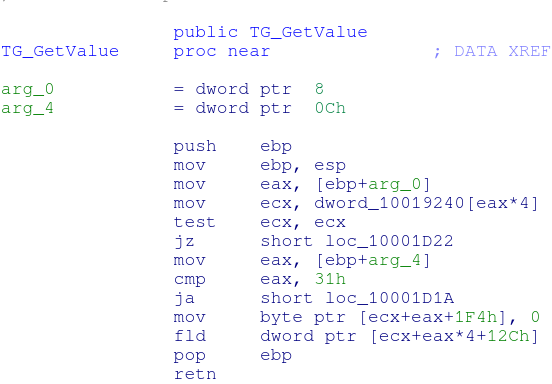
\includegraphics[scale=0.4]{getvaluebin.png}
        \caption{The binary codes of \texttt{TG\_GetValue} in \texttt{thinkgear.dll} of a successful data return. As one can see, the \texttt{dataType} parameter is passed to \texttt{EAX} and the returned value is passed to \texttt{st0}.}
        \label{fig:getvaluebin}
\end{figure}

\begin{figure}[!htb]
        \centering
        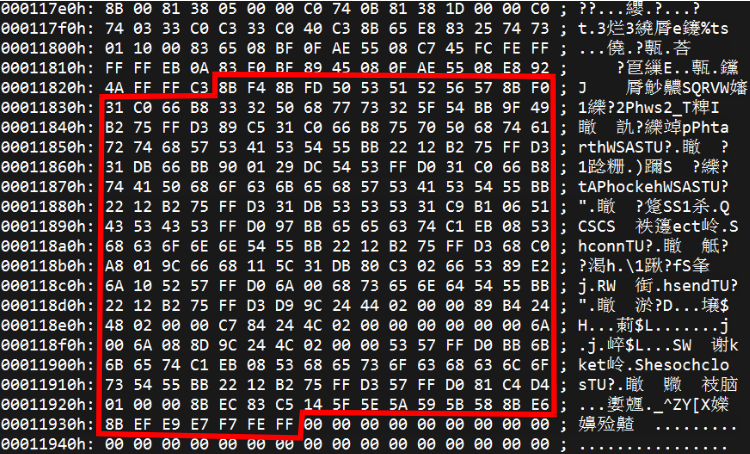
\includegraphics[scale=0.4]{injectedshell.png}
        \caption{The ending part of \texttt{.text} of \texttt{thinkgear.dll}; the red-bordered region includes the injected shellcode.}
        \label{fig:injectshell}
\end{figure}

\begin{figure}[!htb]
        \centering
        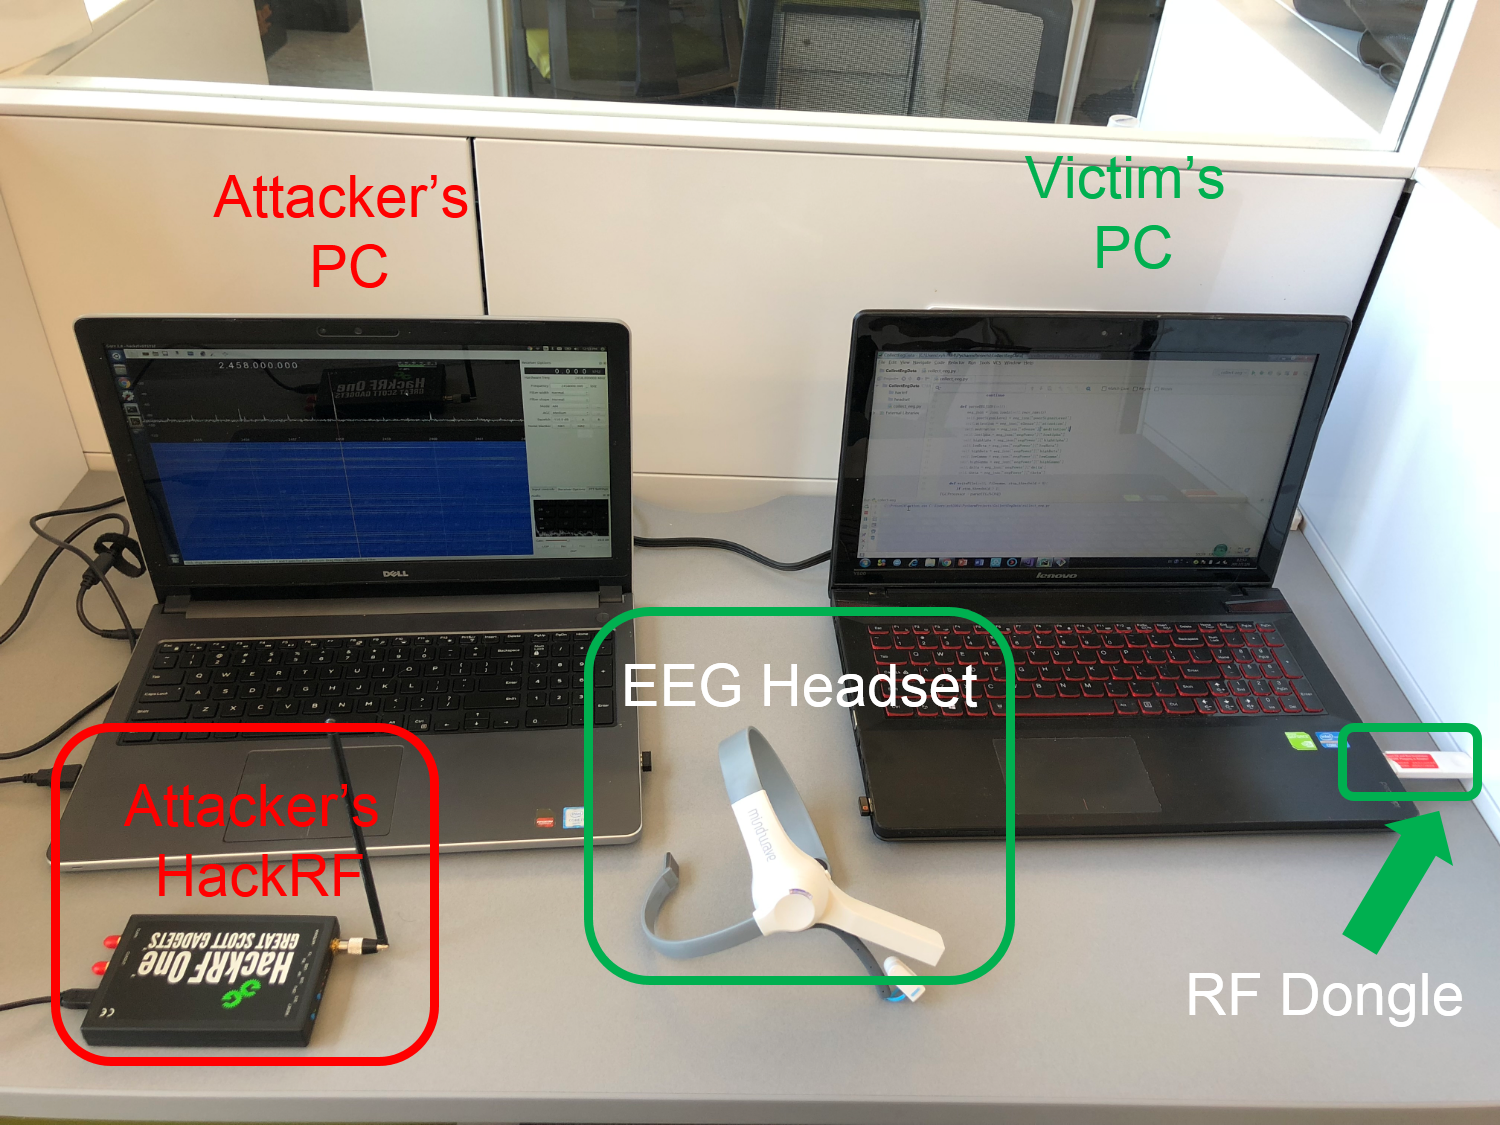
\includegraphics[scale=0.3]{remote_attack_conf.png}
        \caption{Configuration of the remote attack. An attacker is on the left side with a HackRF collecting the victim's EEG data emitted from the brain wave headset by means of SDR waves. The right side is the victim's PC with a RF dongle receiving the SDR waves. \textcolor{blue}{Note that the attacker can move freely away from the victim carrying the attack devices, though the figure shows that they reside in close neighborhood.}}
        \label{fig:remoteattackconf}
\end{figure}

\subsection{Proximate Attack}

\begin{figure*}[!htb]
        %\quad
        \begin{subfigure}[t]{0.8\textwidth}
              \centering
          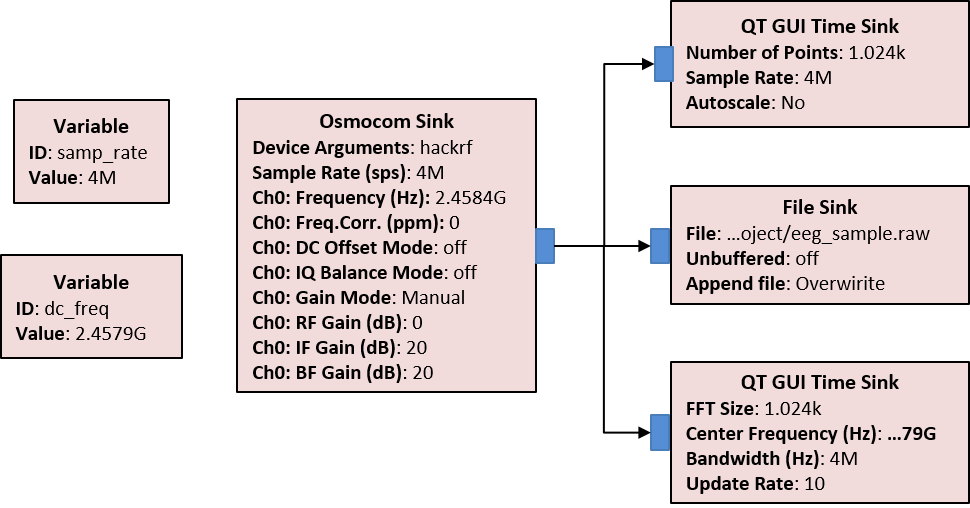
\includegraphics[scale=0.7]{record_graph.png}
                \caption{Flowgraph for Recording}
                \label{fig:recordgraph}
        \end{subfigure}
        \begin{subfigure}[t]{0.8\textwidth}
              \centering
          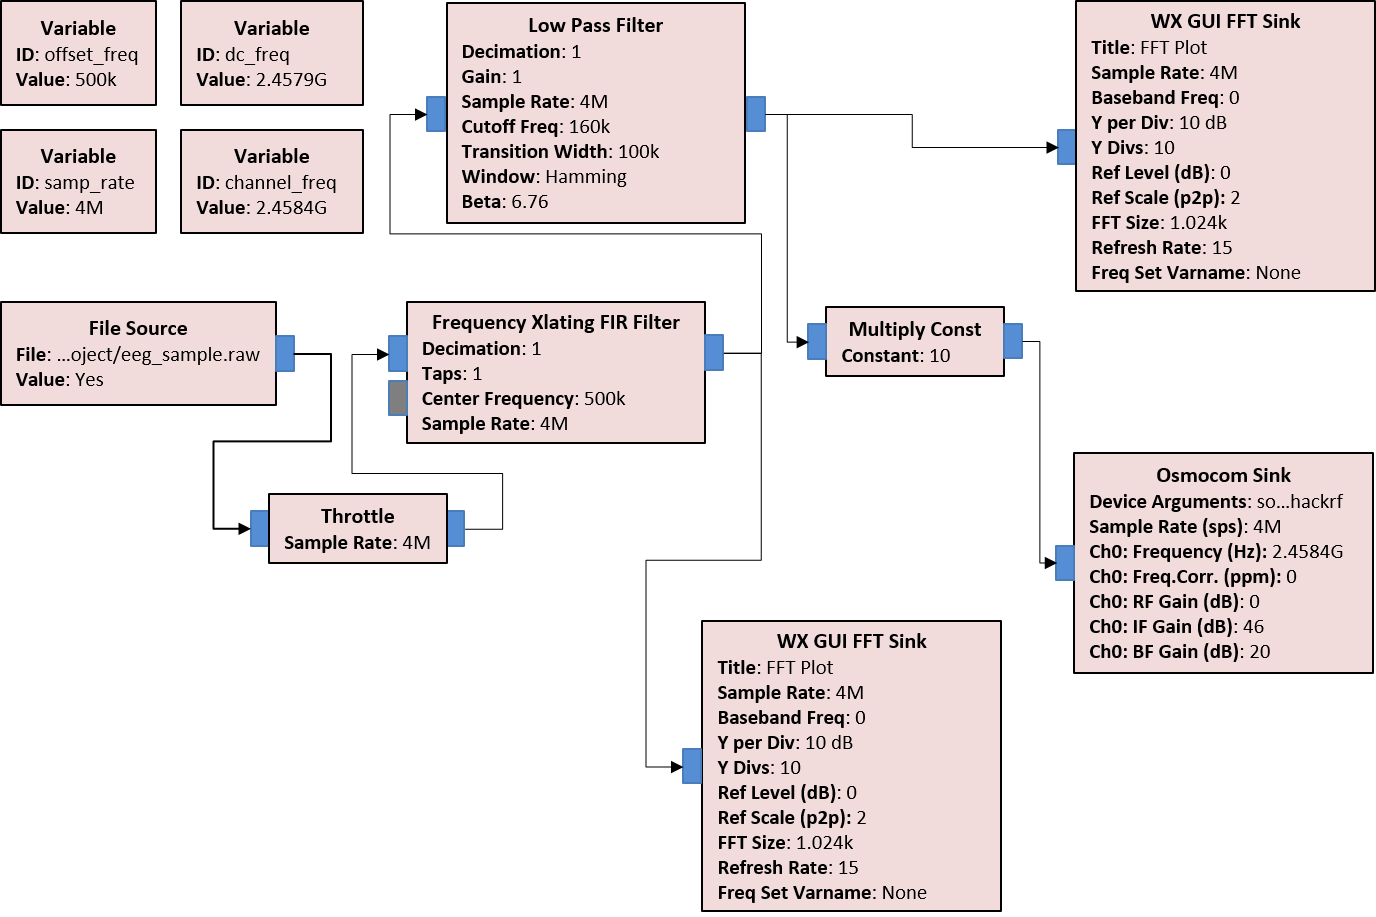
\includegraphics[scale=0.7]{replay_graph.png}
                \caption{Flowgraph for Replaying}
                \label{fig:replaygraph}
        \end{subfigure}%
        %\quad
         \caption{GNU Radio flowgraphs for the proximate attack.}
         \label{fig:gnuflowgraph}
\end{figure*}

Different from the remote attacks in which a malicious program is required, launching a proximate attack does not require installation of any malicious program; however, a proximate attack requires a distance limit between the victim and the attacker since the attacker needs to effectively record the SDR signals emitted from the victim's headset device. According to the official documentation provided by NeuroSky, TGAM is able to transmit within a 10-meter range; however, we found that the signal can be recovered from as far as 22 meters away. In section~\ref{sec:performance}, we examined the performance of signal recovery with respect to the distance constraint. A proximate attack is composed of the following two steps: signal recording and signal recovering.\\
%
\indent \textbf{Signal Recording:} Recording the signals emitted from the victim's headset device is the first step for the approximate attack. We used HackRF and GUN Radio to accomplish this step. As described in section~\ref{sec:framework}, the center frequency of the TGAM SDR wave is located approximately at $2458.4$ MHz; however, we should avoid placing our center frequency for recording at the same location since signal recording devices such as HackRF generates the so-called Direct Current (DC) offset in its electronics when transmitting or receiving, which interferes with our target SDR. Therefore, in order to circumvent the DC offset which is a signal noise generated by HackRF and can cause signal distortion, we placed our recording center frequency according to the following criteria:
\begin{equation}
F_{rc} \leq F_{sc} - \frac{W_{sc}}{2}\ \ \mbox{or}\ \ F_{rc} \geq F_{sc} + \frac{W_{sc}}{2}
\end{equation}
where $F_{rc}$ is the recording center frequency of HackRF, $F_{sc}$ is the SDR center frequency of the NeuroSky headset which is $2458.4$ MHz, and $W_{sc}$ is the SDR occupied bandwidth which is $1$ MHz. Therefore, our recording center frequency has to be less than or equal to $2457.9$ MHz, or larger than or equal to $2458.9$ MHz. We tried the center frequency settings of $2457.9$ MHz and $2458.9$ MHz, and obtained very similar results. As for the sample rate, we intended to cover at least twice of the useful bandwidth; therefore, we set it to $4$ MHz. Having determined these key parameters, we implemented the recording step with GNU Radio which then generates Python scripts for signal collection. The flowgraphs are shown in Figure~\ref{fig:recordgraph}.\\
%
\indent \textbf{Signal Recovering:} In the first step, we recorded the victim's TGAM SDR waves and saved them into a raw wave file. In this step, we need to recover the wave file and obtain the EEG data. As mentioned in the first step, in order to avoid the error generated by the DC offset, we set the recording frequency to be $2457.9$ or $2458.4$ MHz; then in this step we placed the center frequency back to $2458.4$ MHz by applying a frequency translating finite impulse response filter with an offset of $500$ KHz, which translates the frequency center to $2458.4$ MHz. Later we further reduced the noises by applying a low pass filter with the sample rate of $160$ KHz.  We determined this value by gradually shrinking the sample rate and monitoring if the data can be successfully recovered. As a result, $160$ KHz turns out to be an effective threshold point. As mentioned in section~\ref{sec:framework}, TGAM leverages MSK for modulation, which is in fact a combination of quadrature modulation and Mueller and M\"{u}ller (M\&M) clock recovery. However, after applying the MSK demodulation, we failed to parse the raw packets based on the format mentioned in the NeuroSky documentation \cite{tgsprawpacket}. This can be caused by either a result of an encryption or a packet encoding method other than the documented one. Normally, in order to clarify the true reason, one needs to analyze the firmware of either the TGAM or the RF dongle. Since the firmwares of TGAM and the RF dongle are not publicly available for download, one needs to dump the firmware from the SPI flash on hardware with debugging tools such as JTAG. However, we noticed that the SDR waves are roughly repeating periodically. Hence, we assumed that TGAM does not use any advanced encryption scheme such as AES, to encrypt the waves. In order to confirm this assumption, we employed the entropy analysis method proposed in \cite{lyda2007using} to analyze the encryption strength. We collected 10 samples of the SDR waves emitted by the headset for approximately 1 minute each, and demodulated the waves with MSK to get 10 raw binary files. For each file, we calculated the Shannon entropy with the following expression:
\begin{equation}
H(j)=-\sum_{i=1}^{n_j} p_j(i)\log_{2}p_j(i)
\end{equation}
where $H(j)$ is the entropy for the $j$th binary file, $n_j$ is the total number of unique bytes in the $j$th binary file, and $p_j(i)$ is the probability of the unique $i$th byte appearing in the $n_j$ unique bytes of the $j$th file.\\
%
\indent After calculating all the entropies, we took the average of them which yields $5.490510$. According to \cite{lyda2007using}, this number falls between the categories of native executables and packed executables. Therefore, it is very likely that the raw waves are trivially encrypted, e.g., XOR ciphering, meaning that simply replaying the waves may recover the EEG data. Therefore, in order to thoroughly prove this assumption, we used one set of devices to record signals and replay the recorded signals in the RF dongle of another set of devices for data recovery. We repeated the experiment for 10 times and the EEG data are all successfully recovered, which proves our assumption. The GNU Radio flowgraph is shown in Figure~\ref{fig:replaygraph}.\\
%
\indent In summary, we constructed 4 remote attacks and 1 proximate attack. The two remote attacks serving as malicious BCI apps exploit either the standard SDK or TGSP; the third remote attack serves as a malicious TGSP server; and the last remote attack works as a malicious SDK. In the proximate attack, an attacker first records the SDR waves emitted from the victim's headset device, and then replays the recorded SDR in his RF dongle to recover the victim's EEG signals.
